\documentclass[../TDT6.tex]{subfiles}%

\begin{document}
\section{Isothermes d'\textsc{Andrews}}
% \begin{minipage}[t]{.60\linewidth}
\enonce{%
	\begin{wrapfigure}[7]{R}{0.4\textwidth}
		\vspace*{-20pt}
		\begin{center}
			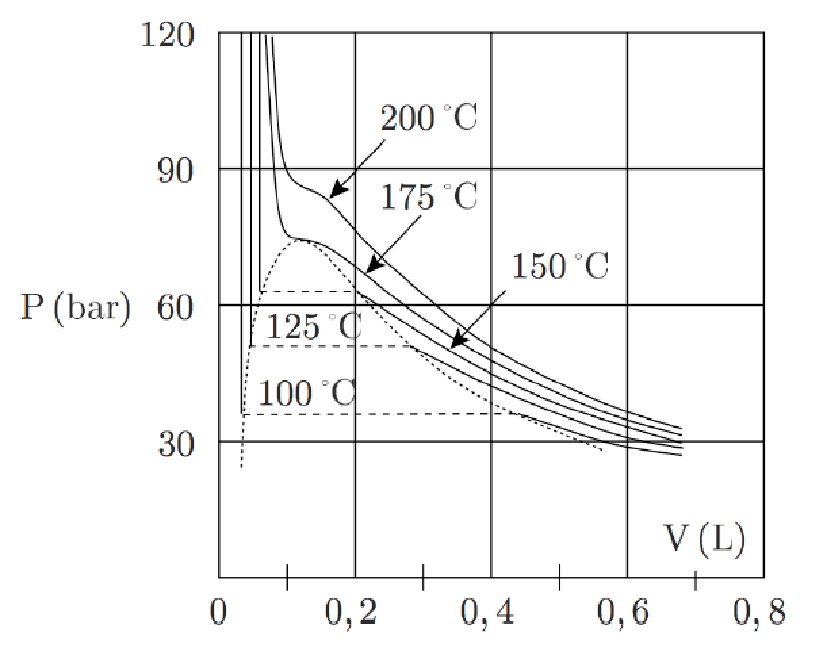
\includegraphics[scale=1]{iso_and}
		\end{center}
	\end{wrapfigure}
	La figure ci-contre représente un ensemble de courbes expérimentales appelées
	isothermes d'\textsc{Andrews}, représentant la pression $P$ d'une mole de
	fluide en fonction du volume \textbf{molaire}, pour différentes températures.
}%
\QR{%
	Déterminer les coordonnées $(P_C,V_C)$ du point critique.
}{%
	\sswitch{
		\hfill
		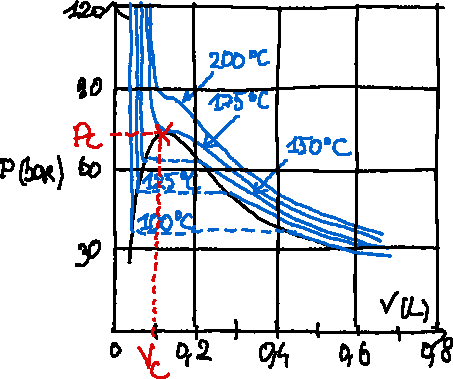
\includegraphics[width=.3\linewidth, valign=t]{iso_and_critique}
		\hspace*{\fill}
	}{
		\leavevmode\vspace*{-15pt}\relax
		\begin{center}
			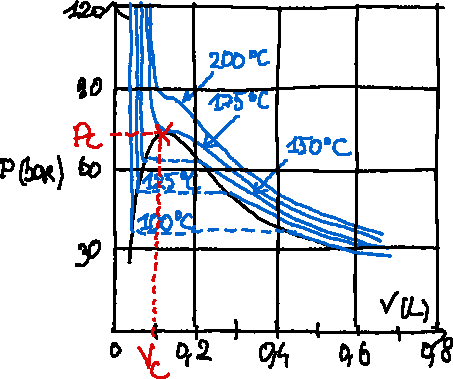
\includegraphics[width=.3\linewidth]{iso_and_critique}
		\end{center}
	}
	\smallbreak
	On lit $V\ind{C} = \SI{0.1}{L}$ et $P\ind{C} = \SI{70}{bar}$.
}%

\QR{%
	Indiquer la courbe de rosée et la courbe d'ébullition.
}{%
	\sswitch{
		\hfill
		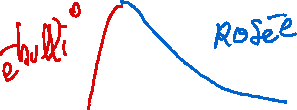
\includegraphics[width=.3\linewidth, valign=t]{iso_and_ebros}
		\hspace*{\fill}
	}{
		\leavevmode\vspace*{-15pt}\relax
		\begin{center}
			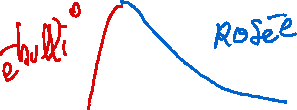
\includegraphics[width=.3\linewidth]{iso_and_ebros}
		\end{center}
	}
}%
% \end{minipage}
% \begin{minipage}[t]{.40\linewidth}
% 	~
% 	\vspace*{-10pt}
% 	\begin{center}
% 		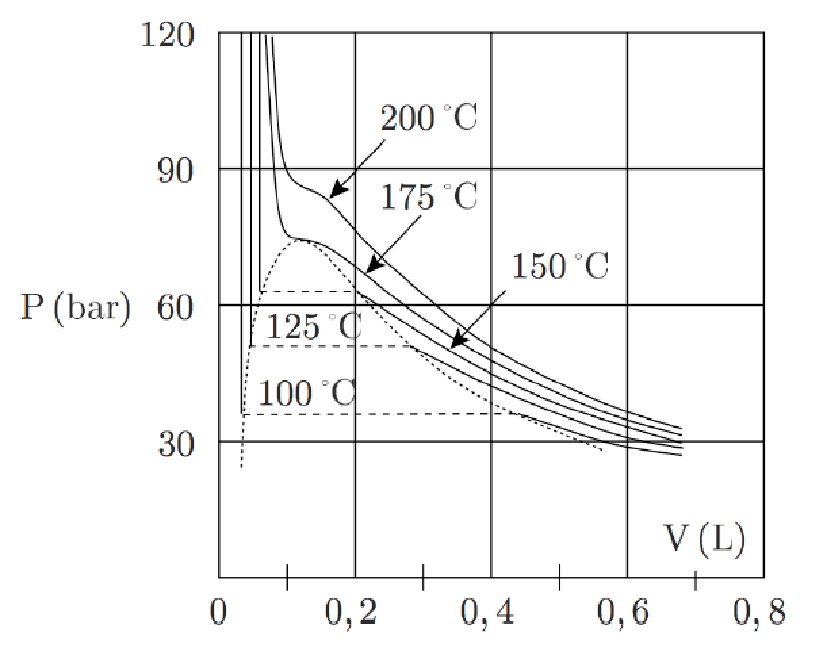
\includegraphics[scale=1]{iso_and}
% 		\label{fig:isoand}
% 	\end{center}
% \end{minipage}


\begin{blocQR}[start=3]
	\item \enonce{%
		Préciser l'état physique et calculer, s'ils sont définis, les titres
		massiques $x_V$ et $x_L$ de la vapeur et du liquide pour~:
	}%
	\QR{%
		$V_m = \SI{0.6}{L.mol^{-1}}$ et $T = \SI{110}{\degreeCelsius}$~;
	}{%
		~
		\smallbreak
		\vspace{-15pt}
		\begin{isd}[interior hidden]
			\begin{center}
				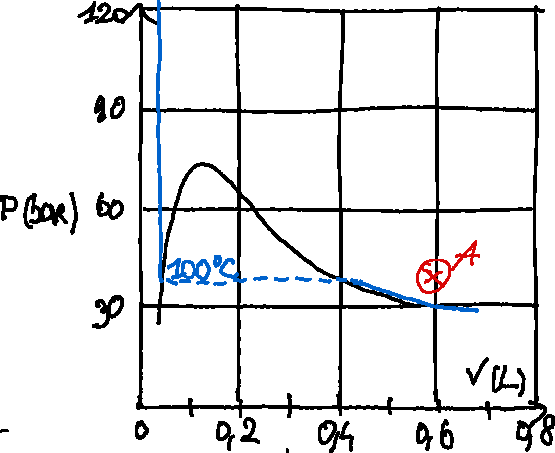
\includegraphics[width=.8\linewidth]{iso_and_06}
			\end{center}
			\tcblower
			Ici, on est dans l'état gazeux car $T\ind{A} < T\ind{critique}$, soit
			$\boxed{x_g = 0}$ et $\boxed{x_{\ell} = 0}$.
		\end{isd}
	}%

	\QR{%
		$P = \SI{110}{bars}$ et $T = \SI{200}{\degreeCelsius}$~;
	}{%
		Dans ce cas, $T\ind{B} > T\ind{critique}$~: $x_g$ et $x_{\ell}$ ne sont pas
		définis~: on est dans l'état du fluide supercritique.
	}%

	\QR{%
		$V_m = \SI{0.2}{L.mol^{-1}}$ et $T = \SI{125}{\degreeCelsius}$.
	}{%
		~
		\smallbreak
		\vspace{-15pt}
		\begin{isd}[interior hidden]
			\begin{center}
				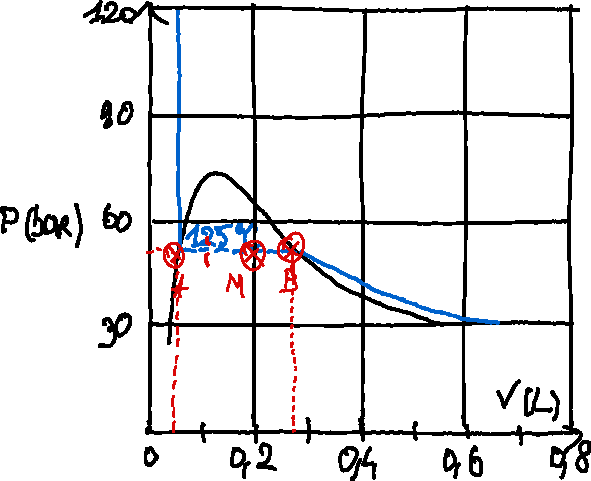
\includegraphics[width=.8\linewidth]{iso_and_02}
			\end{center}
			\tcblower
			On est dans la zone diphasée. D'après le théorème des moments,
			\begin{gather*}
				x_g = \frac{AM}{AB} = \frac{v - v_{\ell}}{v_g-v_{\ell}} = \frac{V_m -
					V_{m,\ell}}{V_{m,g} - V_{m,\ell}}
				\\\qav
				\left\{
				\begin{array}{rcl}
					V_g      & = & \SI{0.28}{L}
					\\
					V_{\ell} & = & \SI{0.05}{L}
					\\
					V        & = & \SI{0.2}{L}
				\end{array}
				\right.\\
				\AN
				\xul{x_g = \num{0.65}}
				\qet
				\xul{x_{\ell} = \num{0.35}}
			\end{gather*}
		\end{isd}
	}%
\end{blocQR}

\QR{%
	Que vaut le volume molaire de la vapeur saturante à la pression de
	\SI{40}{bars}~?
}{%
	Pour lire le volume (molaire) de la vapeur saturante à \SI{40}{bars}, on se
	reporte sur la courbe de rosée, et on lit $\xul{V_m \approx
			\SI{0.4}{L.mol^{-1}}}$.
}%

\end{document}
